% Chapter 2
\chapter{Overlay Network} % Chapter title

This part of the project was done in the same PC as previously explained but in the Windows Operating System with docker toolbox installed having a virtual machine called default running the docker engine, this was done to solve a problem occured by trying to run docker machines. \\

The main problem that appeared in this part of the project on the Ubuntu 14.04 dual boot was that the kernel module failed to load,  therefore I had use the Windows Operating System.\\

I had to turn on the hardware virtualization in the BIOS since docker has to have access to the core of the computer for running virtual machines and containers.\\

For each container I added the basic configuration of a container using the repositories with the minimal configuration of OpenStack in the docker hub.\cite{8} \\

After adding this configuration I logged in to each docker container to add the components that OpenStack needs to create a Networking environment for self Service Networks information that I found in the OpenStack documentation\cite{9} \\

This part of the configuration is done because we want all the components to be virtualized and self dependent, for future developement of the project and for migration of the environment.\\

If we have an environment that is not dependent of the hardware properties the provisioning of the services in terms of scalability and availability increase considerably.\\

\section{Overlay Network interface in OpenStack and Docker} 

OpenStack has to be configured to use firewall, Load balancer, routers, switches, GRE tunnels and VXLAN protocols as specified in the self-service network configuration.\\

OpenStack as well as Docker containers use namespaces for networking meaning that a container with the same specifications can be given a different namespace with the same configuration, increasing the scalability of a system, the availability by replicating and the resilience by duplicating the containers for prevention of a possible failure, and without losing communication with its dependencies.\\

As shown in the first part of the project this namespaces are stored in a database for the network discovery.\\

Overlay interface: 10.0.1.0/24 which we will be using in the docker compose or creations of virtual machines.\\

\begin{lstlisting}[language=bash,frame=tb,caption={OVS configuration in OpenStack}]
[ovs]
bridge_mappings = provider:br-provider
local_ip = 10.0.1.0/24
[agent]
tunnel_types = vxlan
l2_population = true
[securitygroup]
firewall_driver = iptables_hybrid
\end{lstlisting}\\

Following the steps of the configuration after all the containers where configured:
for the docker daemon to be available, the default virtual machine must generate TLS certificates, to secure all communications between the servers and the web browsers.\\\

Then I created the Dockerfile and dependencies and deployed the configuration:\\

\begin{lstlisting}
$docker-machine regenerate-certs default
$docker-machine restart default
$eval $(docker-machine env default)
$docker build -t <image_name>.
<dot> specifies that configuration files are located in the current directory
$docker images # to check the image is created.
\end{lstlisting}


Running the app in my physical host: \\
\begin{lstlisting}
$docker run –p <Host_port>:<container_port> <image_name>
\end{lstlisting}
\\

\section{Docker containers inside of virtual machines}

This part of the project explains the simulation of a clustered environment, and it was don for two main reasons.\\

First to balance the load of the containers from one virtual machine to other virtual machines, creating a resilient environment.

And second to check how the overlay plugin works to add to the configuration of the SDN environment with OpenvSwitch.\\

For the creation of this docker provides docker-compose files which are files written in yaml language having all the descriptions for a creation of a virtual machine such as number of cpu's, network driver used, the services or containers that are going to run in this machine, etc.\\

First  I created the docker-compose file that it is used for running various container applications at once this information I learned in the docker documentation an example of my OpenStack configuration it is attached as docker-compose.yml in myvm1.\\

Next I started a virtual machine on docker using the virtualbox driver and copied the docker-compose file in the virtual machine and then I deployed the services.\\  

\begin{lstlisting}
$docker-machine create –-driver virtualbox myvm1
$docker-machine scp docker-compose.yaml myvm1:~
$docker-machine ssh myvm1 ''docker stack deploy -c''
\end{lstlisting}

Attached in the apendix is \autoref{fig:compose} which is an example of the docker-compose file.

\section{Docker Overlay network}

To understand how Docker works from the core of the overlay network I created an environment to store each of the containers in different virtual machines, and I started creating a cluster called Swarm in docker.\\

Docker uses a plugin for the network configuration called overlay, with the architecture to cover the multiple virtual machines.\\ 

\section{Cluster}

A service cluster is a multiple number of servers that communicate with each other to provide service to clients. A cluster provides high availability, scalability reliability to a system in any case of failure; if a server shutdown somehow the service won’t stop serving but instead it will distribute the workload to other servers.\\

Swarms are a group of machines that are joining the cluster in docker. After a machine joins a swarm the node that joins the cluster will provide resilience, since at the beginning there was a single point of failure.\\

Now having two nodes in a cluster, if one node goes down the other node that will have all the data needed to perform any actions will respond for the call that had to be answered by the node that went down.\\

\subsection{Minimal number of nodes}

It is very important that the master eligible nodes do as little work as possible since master nodes can behave as a controller nodes.\\

The minimum number of master eligible nodes in order to join a cluster must be 2 and the most appropriate at the moment of building an infrastructure follows the split brain prevention theorem:\\

The minimum number of master eligible nodes in order to join a cluster must be 2 and the most appropriate at the moment of building an infrastructure follows the next equation:
\begin{equation}
(master\_elegible\_nodes / 2)+1
\end{equation}

In order to explain this, lets suppose a case when there are 3 nodes in the cluster and there is a network failure.\\
\begin{itemize}
\item In the \texttt{First case} if there is only a master node as soon as the two parts of the cluster are not communicating each other they cannot find the master node and choose themselves as a master creating a split brain, and when joining the cluster for the second time  one of this master eligible nodes will have to be restarted loosing all its information.
\item In the \texttt{Second case} if the minimum master nodes is 2, one of the nodes wont see another master eligible node so it wont be able to choose itself as a master node, when the communication is restored it can join again the cluster and work normally 
\end{itemize}

\subsection{Number of nodes in OpenStack}
In OpenStack it is established in the configuration files the quorum which it must be a number higher than \begin{equation}
floor(n/2) + 1 
\end{equation} to avoid split brain\cite{10}

\subsection{Docker cluster}

To check how to develop a cluster with docker containers inside, I added the configurations of an app written in python and the docker file, to deploy the application.\\

In this section I added a box with an app that displayed the number of times a visitant entered to the page and the id of each container after refreshing the page, adding 5 replicas of the same container among 2 virtual machines exposing to the port 80; and a visualization of the containers spread along the virtual machines exposed to port 8080.

\paragraph{Why do we need load balance of containers?}\\

The heavy loaded servers and multiple computations that need to be executed leads to the problem of directing the containers in the correct virtual machines for the correct performance and an efficient usage of resources.\\

Therefore docker provide load balance of docker containers with the multi-host networking, next explained.\\

\section{Multi-Host networking, load balance of containers in VMs and docker cluster}\\

For multihost networking, docker provides the overlay network driver, but in difference to the normal architecture for docker containers with bridges, the overlay driver needs either a docker engine running in swarm mode or a cluster of hosts using a key value store. \\

To create a new network driver first I created the cluster with the key value store. The key value have the network state information, endpoints, IP addresses, etc.\\


For this 2 machines have been created while one is the master, \autoref{fig:master} presents the virtual machines created with the master node represented by a "*" and the other nodes that joined the cluster, we can see the default node as well which contains the docker engine configuration\

\begin{figure}[bth]
{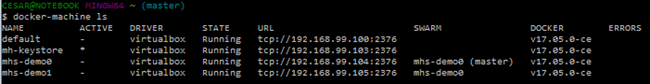
\includegraphics[width=1\linewidth]{gfx/master}}\caption[Master node and slaves in Docker]{Master node and slaves in Docker}
{\label{fig:master}
\end{figure}

For the overlay network:
\begin{lstlisting}
$ eval $(docker-machine env --swarm mhs-demo0)
$ docker network create --driver overlay --subnet=10.0.1.0/24 my-network
\end{lstlisting}

Creating the network configuration: \autoref{fig:outside} shows the configuration of the links between docker machines and the created overlay network called my-network for the intercommunication between docker-machines that have inside docker containers.\\

\begin{figure}[bth]
{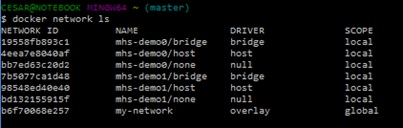
\includegraphics[width=1\linewidth]{gfx/outside}}\caption[Network overlay configuration]{Network overlay configuration}
\label{fig:outside}
\end{figure}

In the appendix \autoref{fig:demo0} and \autoref{fig:demo1} shows the configuration of the 2 virtual machines created demo0 and demo1 both hosts are running with the same network id, the same of my-network network, meaning that the multihost network is ready. Next for running an application we need to change the environment to the swarm master and run containers from the master and not from the slaves.\\

This configuration works in the next way: \\

First the mh-keystore is the master node of the configuration, all the instructions that we want to give such as location of the containers within the clusters or the number of replicas that we would like to add for the resilience of the service is given by this master node.\\

The assignment of master and slaves is helpful for the distribution of the data, the master node will have all the information about containers and how do they work, and the slaves will operate and run each particular service.\\


Following the steps of this configuration but implementing OpenvSwitch to the infrastructure to meet the SDN model the service must be isolated.\\

For this it would be very useful to create a container with all the modules and services that are needed to run OpenStack, since containers have all the inter-process communications within the container itself, the computations will be executed inside of the container and it will become a more portable infrastructure.\\

\section{OpenvSwitch configuration for a container deployment}

This part of the project was applied to implement an isolation of the networking component.\\

Because OpenvSwitch is the one that will have all the configuration and information of the location of each container.\\

First in boot2docker which is the virtual environment in which docker is working (we may think of it is as the virtual machine manager), we need to enable the OpenvSwitch kernel module as explained in the architecture of OpenvSwitch in previous sections.\\

Then adding the configuration for the connectivity of the containers as it was shown in the first chapter with the OpenvSwitch.\\

This configuration will be saved after commiting the container, but the configuration of the virtual environment must be previously added manually in every environment.\\
\\

\begin{lstlisting}
modprobe openvswitch
docker run –itd –-cap-add NET_ADMIN socketplane/openvswitch
docker exec <container id ovs> ovs-vsctl add-br s1 
\end{lstlisting}

Note: It is important to notice that I had to do this with my virtual environment since I was using Boot2docker in windows.

\section{Problems and Solutions}

As previously explained in the use of swarm node, the docker toolbox for windows uses swarms to add the docker engine to the nodes.\\

Since the docker engine is the one in charge of the management and storage of information such as process id and state of the containers, in the next chapter because the migration of the containers must be an independent architecture detached from the operating system we need the docker engine to work as a manager for this connections therefore for the next part of the project I will not be able to use the docker toolbox for Windows